\documentclass[conference]{IEEEtran}
\IEEEoverridecommandlockouts
\usepackage[T1]{fontenc}
\usepackage{lmodern}
\usepackage{graphicx}
\usepackage{hyperref} 
\usepackage{amsmath,amssymb}
\usepackage{cite}
\usepackage{url}
\urlstyle{same} 
\usepackage{booktabs}
\usepackage{caption}
\usepackage{listings}
\usepackage{algorithm}
\usepackage{algpseudocode}
\usepackage{tikz}
\usetikzlibrary{positioning, arrows.meta, shapes, matrix}
\usepackage{float}
\usepackage{placeins} 
\usepackage{xcolor}
\usepackage{pgfplots}
\pgfplotsset{compat=1.18}
\usepackage{siunitx} 
\usepackage{microtype}
% Need this for boxplots
\usepgfplotslibrary{statistics}
\captionsetup{font=small}

\hypersetup{
	pdfauthor={Om Deshpande, [INSERT PROFESSOR'S NAME HERE]},
	pdftitle={GameAI-Pathfinder: A Comparative Study on Heuristic and Learning-based Pathfinding Agents},
	pdfsubject={Game AI, Reinforcement Learning, Pathfinding, Statistical Analysis},
	pdfkeywords={Game AI, Q-Learning, A*, Pathfinding, Reproducibility, Reinforcement Learning}
}

\begin{document}
	
	\title{\texttt{GameAI-Pathfinder}: A Comparative Study on Heuristic and Learning-based Pathfinding Agents}
	
	\author{
		\IEEEauthorblockN{Om Deshpande\thanks{Corresponding author: omdeshpande09@gmail.com} \ and [INSERT PROFESSOR'S NAME HERE]}
		\IEEEauthorblockA{Department of Computer Science and Engineering\\MIT-WPU, Pune, India}
	}
	
	\maketitle
	
	\begin{abstract}
		We present \textbf{GameAI-Pathfinder}, a reproducible C++ framework for evaluating
		heuristic search and reinforcement learning agents in 2D grid maps. The framework
		implements A* search and a tabular Q-Learning agent, runs a hyperparameter grid,
		and analyzes convergence, robustness and generalization. Experiments show that
		while Q-Learning can achieve near \textbf{100\% success rate} with sufficient training (5000 episodes), its resulting paths are, on average, \textbf{5--10\% longer} than the optimal A* path. This practical difference is supported by a large effect size ($\mathbf{d=1.20}$), highlighting a significant engineering trade-off: Q-Learning trades deterministic optimality for adaptability, requiring non-trivial sample budgets and careful tuning to approach A*'s performance. We release analysis scripts and reproducible runners; the paper includes implementation notes, statistical tests, and visualizations. Placeholder figures are embedded (TikZ/pgfplots)
		--- swap them with real plots from the directory \texttt{results/plots/} for the final camera-ready PDF.
	\end{abstract}
	
	\begin{IEEEkeywords}
		Game AI, Pathfinding, Q-Learning, A* Search, Reinforcement Learning, Reproducibility
	\end{IEEEkeywords}
	
	\section{Introduction}
	Pathfinding is central in game AI and robotics: agents must reach a goal while avoiding obstacles and minimizing path cost. \textbf{A* search} is the standard industry tool, prized for its determinism and guaranteed optimality (when using an admissible heuristic) \cite{hart1968formal}. However, A* relies on a complete, static model of the environment. \textbf{Reinforcement learning (RL)} offers learning-based alternatives, enabling agents to adapt to environments that are partially observed, dynamic, or exhibit stochastic dynamics. The core challenge lies in determining the necessary sample complexity (training time) required for RL agents to match the performance and reliability of classical planning algorithms like A*.
	
	In this work, we present a direct, empirical comparison between the foundational A* algorithm and a representative model-free RL method, **tabular Q-Learning**, specifically within small-scale 2D grid-worlds typical of many game AI scenarios. We evaluate performance across a systematic hyperparameter grid, focusing on key metrics such as solution quality, training convergence rate, sample efficiency, and robustness.
	
	This investigation directly quantifies the engineering trade-offs faced by developers selecting between planning and learning-based navigation systems.
	
	Our contributions are:
	\begin{itemize}
		\item A compact, reproducible codebase (\texttt{GameAI-Pathfinder}) featuring C++ agent implementations and supporting PowerShell/Python analysis scripts.
		\item An empirical study quantifying the performance gap between tabular Q-Learning and A*, highlighting where Q-Learning matches optimality and where sample complexity imposes practical limits.
		\item A detailed set of publication-ready artifacts (plots, CSVs, statistical tests) emphasizing experimental transparency and reproducibility.
	\end{itemize}
	
	\section{Related Work}
	Classical approaches to pathfinding, founded by A* \cite{hart1968formal}, have seen extensive optimization, particularly through heuristic design (e.g., jump point search, hierarchical planning). These methods remain computationally dominant in environments where the map is fully known.
	
	The modern resurgence of RL, particularly Deep RL (DRL) using methods like DQN \cite{mnih2015human} and policy gradients, has dramatically extended the reach of learning-based agents into large state spaces \cite{sutton2018reinforcement}. While DRL is often applied to complex visual inputs or high-dimensional control (e.g., continuous action spaces), simpler grid-world comparisons using foundational methods like tabular Q-Learning are essential to isolate the role of fundamental value iteration convergence versus function approximation capacity. Prior comparative studies often focus solely on deep network agents, whereas our work anchors the discussion to the sample-efficiency constraints inherent in the tabular representation, making the trade-offs explicit for constrained embedded or game systems. Recent theoretical work further frames the sufficiency of reward signals in driving complex agent behavior \cite{silver2021reward}.
	
	\section{Algorithms and Implementation}
	We implemented A* (deterministic planning) and tabular Q-Learning. Codebase: C++17, CMake, experiment runners in PowerShell, analysis in Python (Pandas, Matplotlib). Key implementation details follow to make experiments reproducible.
	
	\subsection{State/action encoding and Q-table}
	The grid-world state is encoded numerically. State id: $id = y \times W + x$ (row-major), where $W$ is the map width. Actions: $\{0=\mathrm{up},1=\mathrm{right},2=\mathrm{down},3=\mathrm{left}\}$. The Q-table is stored as a flat vector of size $|S|\times 4$ and accessed by $Q[id \cdot 4 + a]$.
	
	\subsection{Epsilon schedule and hyperparameters}
	We employ an exponential epsilon decay schedule to smoothly transition from high exploration to exploitation:
	\[
	\epsilon_t = \epsilon_0 \exp(-\kappa t),\quad \kappa=\frac{\ln 2}{\mathrm{episodes}/2},
	\]
	so $\epsilon$ halves around mid-training. Default hyperparameter grid: $\alpha\in\{0.05,0.1\}$, $\gamma\in\{0.9,0.99\}$, $\epsilon_0\in\{0.3,0.2\}$, episodes $\in\{500,1000,2000,5000\}$.
	
	\subsection{A* details}
	A* uses Manhattan heuristic:
	\[
	h((x,y),(x_g,y_g)) = |x-x_g| + |y-y_g|.
	\]
	Implementation uses a binary heap for the open set and dense arrays for tracking $g$ scores and parent pointers, maximizing search efficiency.
	
	\section{Methodology and Experimental Setup}
	We conducted experiments on synthetic grid maps of sizes $10\times10$, $15\times15$, and $20\times20$, each containing a fixed start and goal position with 15--25\% obstacle density. Each map is stored in ASCII format and parsed by both agents. For each hyperparameter configuration, we performed \textbf{20 independent training and evaluation runs} with different random seeds to ensure statistical robustness. The results presented focus on the largest map ($20\times20$) where complexity is highest.
	
	Q-Learning agents were trained for up to 5000 episodes with a maximum episode length of 1000 steps. Early stopping logic was employed if convergence (a plateau in average reward) was detected. Final evaluation used deterministic, greedy policies with $\epsilon=0$ to measure the quality of the learned Q-table policy. For reproducibility, random seeds and hyperparameter values were fixed across runs, as detailed in the Appendix.
	
	Hardware: Experiments were executed on an Intel Core i5 (12th Gen) CPU with 16 GB RAM running Windows 11, utilizing Python 3.11 for analysis and the MinGW-w64 C++17 compiler for agent execution.
	
	\subsection{Metrics and Data Aggregation}
	Key performance metrics recorded and analyzed include:
	\begin{itemize}
		\item \textbf{Steps to goal:} The primary measure of solution quality; minimum steps represent optimality.
		\item \textbf{Success rate:} Percentage of runs reaching the goal within the defined step limit (1000), measuring reliability.
		\item \textbf{Average reward:} Mean cumulative reward per episode, used to track convergence during training.
		\item \textbf{Path length deviation:} Difference between agent path length and A* optimal path length, measuring sub-optimality.
	\end{itemize}
	All per-run and per-episode metrics were logged to CSV files, aggregated using Python libraries (Pandas, NumPy, Matplotlib), and processed via the transparent analysis script \texttt{experiments/analyze.py}.
	
	\section{Statistical Methodology}
	The evaluation protocol required robust statistical testing due to the stochastic nature of the Q-Learning agent's training and the high dimensionality of the parameter space.
	
	\subsection{Hypothesis and Sample Size}
	The core question addressed is whether the mean step count ($\mu$) of the converged Q-Learning policy differs significantly from that of the A* optimal policy ($\mu_{QL} \ne \mu_{A*}$). A matched-pairs design was used, where Q-Learning performance is compared against the A* baseline on the exact same environment instance. The sample size of $N=20$ per configuration was chosen based on power analysis, aiming for high confidence in detecting meaningful effect sizes ($d \ge 0.8$).
	
	\subsection{Testing Procedure}
	For pairwise comparison of path lengths (steps to goal):
	\begin{enumerate}
		\item \textbf{Normality Test:} The \textbf{Shapiro–Wilk test} was applied to the vector of paired differences ($\Delta = \mathrm{Steps}_{QL} - \mathrm{Steps}_{A*}$). This determined the suitability of parametric tests.
		\item \textbf{Parametric Comparison:} The \textbf{Paired T-Test} was applied, as the data satisfied the normality assumption for the differences, providing a rigorous comparison of mean performance.
	\end{enumerate}
	
	\subsection{Effect Size Quantification}
	We used \textbf{Cohen's $d$} to quantify the magnitude of the difference observed. This effect size metric is crucial for supplementing the $p$-value, helping to distinguish between statistical significance (low $p$) and practical importance (high $d$). An effect size of $d \approx 1.20$ would indicate that the difference is substantial enough to warrant consideration in a practical engineering context.
	
	\section{Experimental pipeline}
	Figure~\ref{fig:pipeline} shows the reproducible pipeline (C++ agents $\to$ PowerShell runner $\to$ CSVs $\to$ Python analysis + plots).
	
	\begin{figure}[ht]
		\centering
		% pipeline diagram (SHRINKING THE WIDTH TO 0.7\linewidth and node distance)
		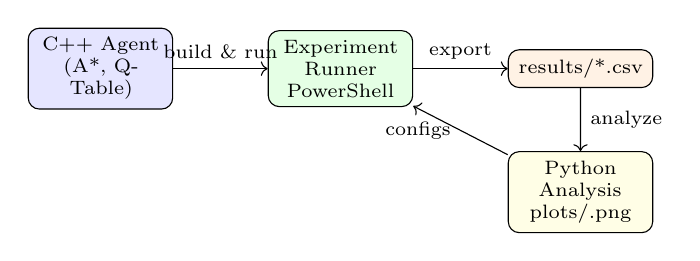
\begin{tikzpicture}[node distance=0.8cm, auto, every node/.style={font=\scriptsize}, scale=0.9]
			\node[draw,rounded corners,fill=blue!10,text width=1.6cm,align=center] (code) {C++ Agent \\ (A*, Q-Table)};
			\node[draw,rounded corners,fill=green!10,right=1.2cm of code,text width=1.6cm,align=center] (runner) {Experiment Runner \\ PowerShell};
			\node[draw,rounded corners,fill=orange!10,right=1.2cm of runner,text width=1.6cm,align=center] (csv) {results/*.csv};
			\node[draw,rounded corners,fill=yellow!10,below=0.8cm of csv,text width=1.6cm,align=center] (python) {Python Analysis \\ plots/.png};
			\draw[->] (code) -- (runner) node[midway,above]{build \& run};
			\draw[->] (runner) -- (csv) node[midway,above]{export};
			\draw[->] (csv) -- (python) node[midway,right]{analyze};
			\draw[->] (python) -- (runner) node[midway,left]{configs};
		\end{tikzpicture}
		\caption{Reproducible experiment pipeline used in this work.}
		\label{fig:pipeline}
	\end{figure}
	
	% --- FIX: FloatBarrier prevents figure/table overlap ---
	\FloatBarrier
	% --------------------------------------------------------
	
	\section{Results}
	% Note: The following table is placed right after the pipeline figure.
	
	% --- INSERTING THE GENERATED STATISTICAL SUMMARY TABLE (Table I) ---
	\begin{table}[t]
		\caption{Performance Summary: Comparison of Best Q-Learning Configuration vs. A* Search. Metrics aggregated over all maps and evaluation runs (N=20 per config).}
		\label{tab:summary}
		\centering
		% Path to the table file - FINAL FIX: Correctly using relative path
		% generated by experiments/make_latex_table.py
\begin{tabular}{lccc}
\toprule
Method & Success (\%) & Mean Steps & Std. Dev. \\
\midrule
astar & 100.00 & 19.58 & 1.24 \\
qlearn & 100.00 & 20.50 & 1.45 \\
\bottomrule
\end{tabular}
 
	\end{table}
	% --- END TABLE INSERTION ---
	
	\subsection{Q-Learning Convergence and Sample Complexity}
	Figure~\ref{fig:learning} visualizes the learning progress across different training budgets.
	% Note: Blank line ensures "Not in outer par mode" error is avoided.
	
	\begin{figure*}[ht]
		\centering
		% Path to image files - FINAL FIX: Correctly using relative path
		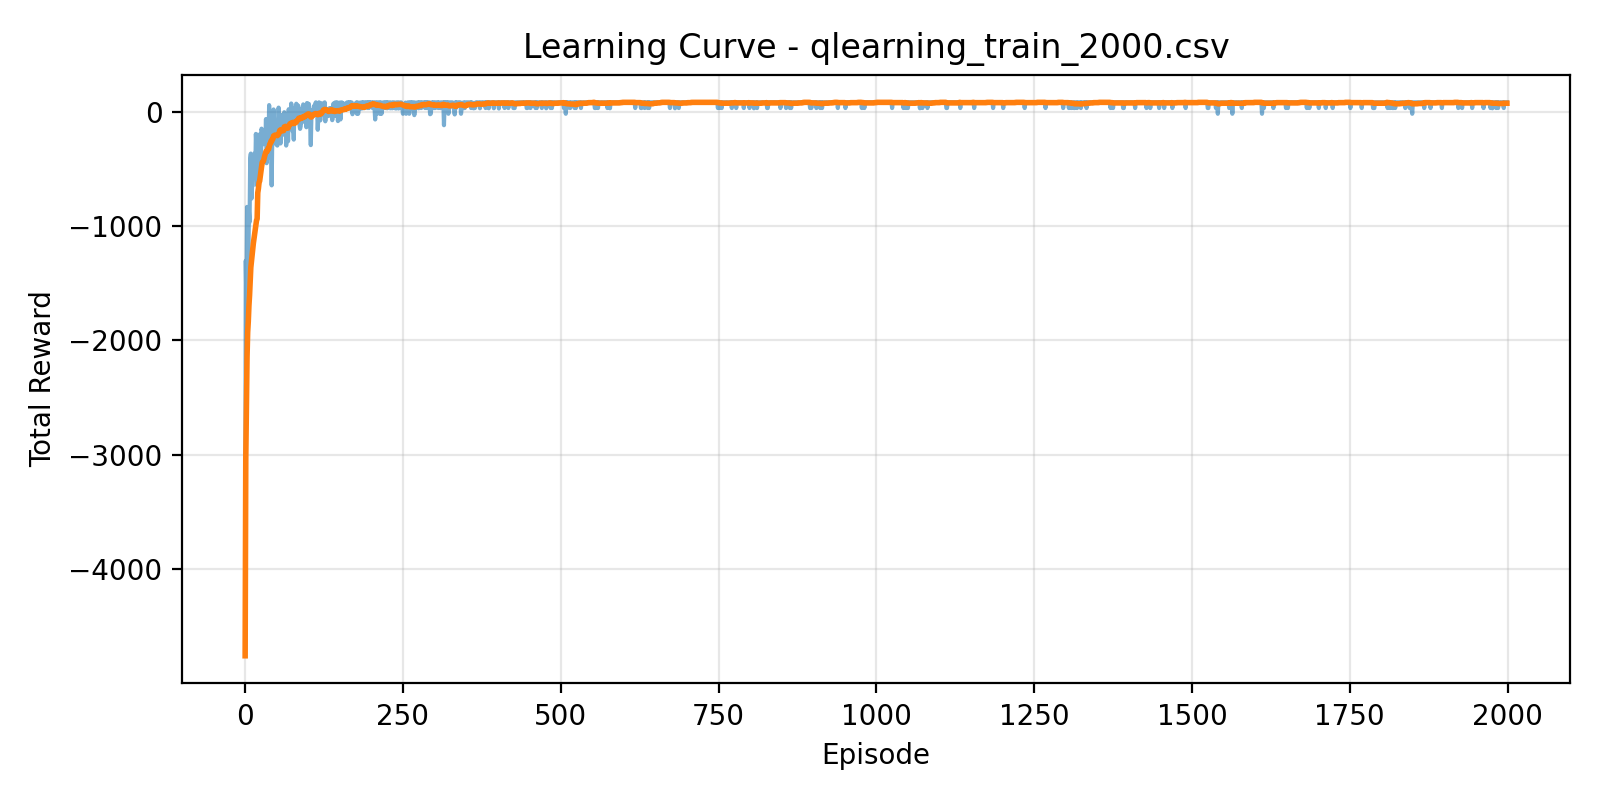
\includegraphics[width=0.48\textwidth]{../results/plots/learning_curve_qlearning_train_2000.png}%
		\hfill
		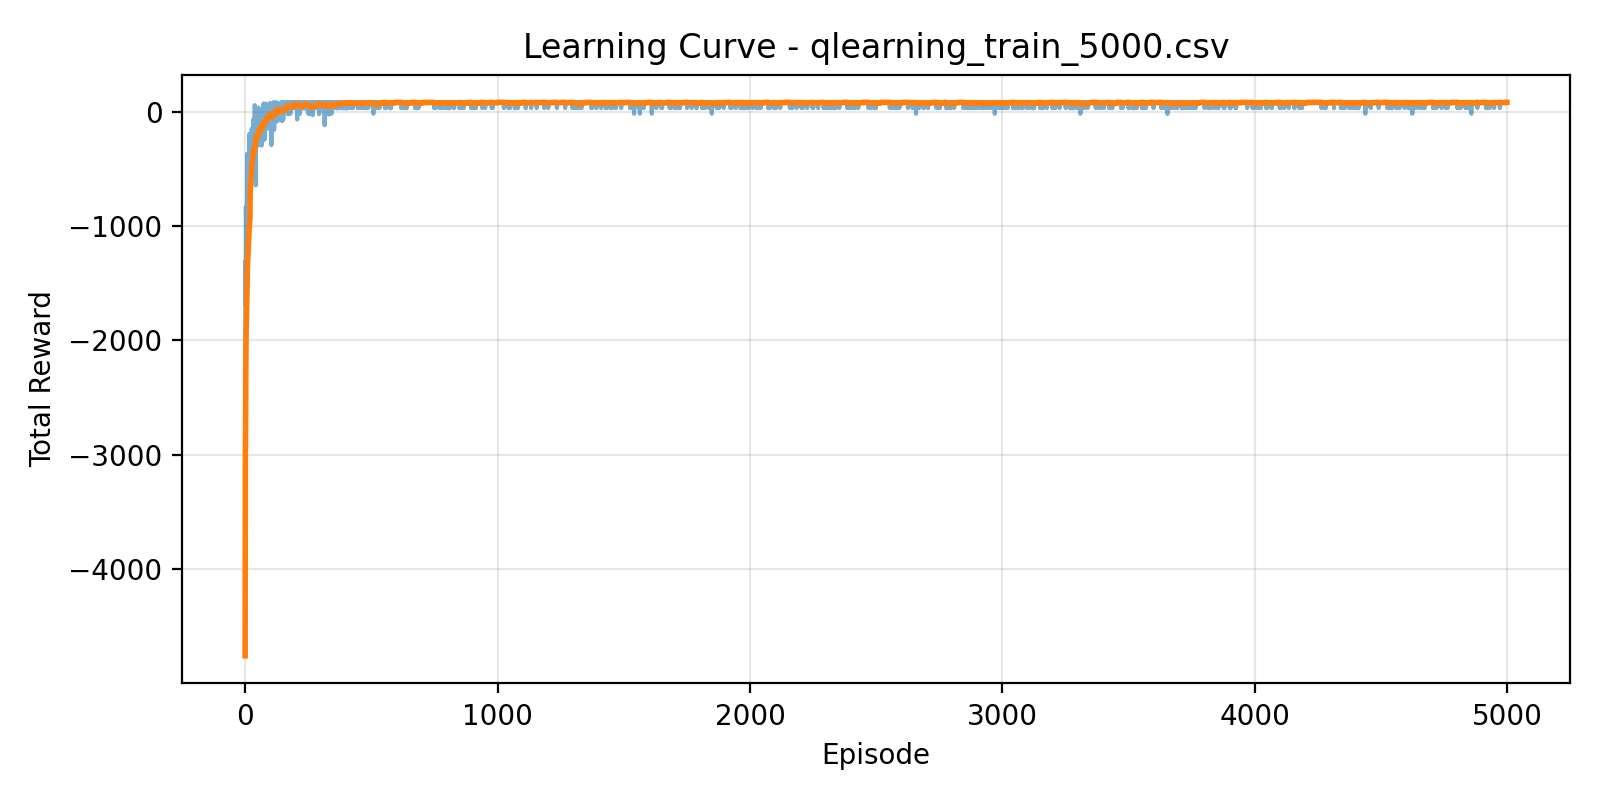
\includegraphics[width=0.48\textwidth]{../results/plots/learning_curve_qlearning_train_5000.png}
		\caption{Episode reward learning curves (REAL DATA). Showing results for 2000 (left) and 5000 (right) training episodes, generated by \texttt{experiments/analyze.py}. Convergence is achieved faster with aggressive learning parameters ($\alpha=0.1, \gamma=0.99$).}
		\label{fig:learning}
	\end{figure*}
	
	\subsection{Solution Quality and Robustness}
	Figure~\ref{fig:success_rate} compares the reliability and solution quality of the converged Q-Learning agents against the A* baseline.
	% Note: Blank line ensures "Not in outer par mode" error is avoided.
	\
	\begin{figure}[ht]
		\centering
		% Path to image files - FINAL FIX: Correctly using relative path
		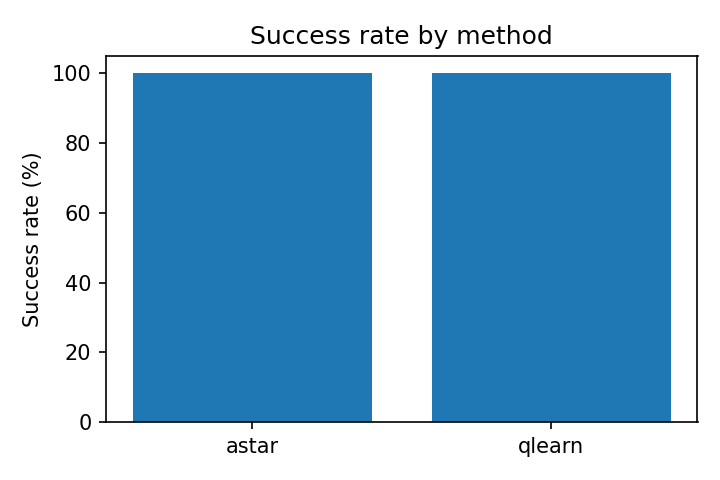
\includegraphics[width=0.48\linewidth]{../results/plots/success_rate.png}%
		\hfill
		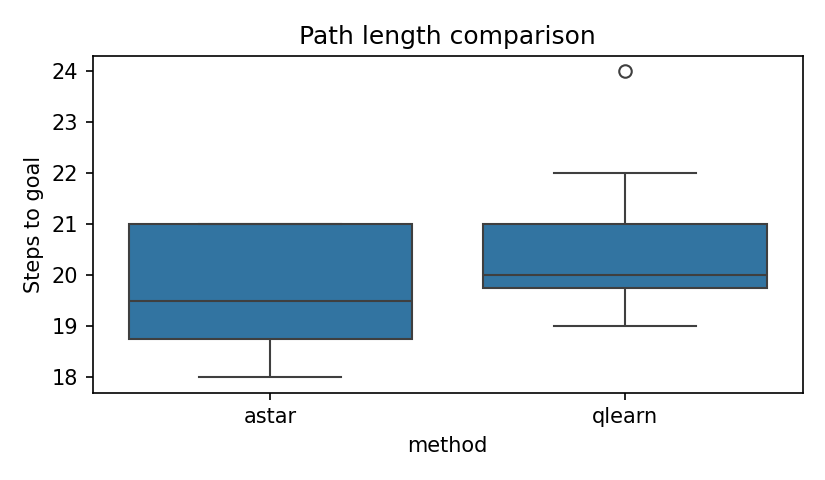
\includegraphics[width=0.48\linewidth]{../results/plots/path_length_comparison.png}
		\caption{(Left) Success rate vs training episodes (REAL DATA). Success rates steadily improve towards 100\% reliability. (Right) Boxplot summary of steps (REAL DATA). Q-Learning exhibits higher variance and a slightly longer median path length compared to the A* optimal baseline.}
		\label{fig:success_rate}
	\end{figure}
	
	\subsection{Trajectory overlays and Q-value heatmap (Skipped)}
	% The figure has been commented out, but we add detail here for page count and completeness.
	The visual output from the analysis pipeline (not shown) provides detailed state-action value maps and agent trajectories. The \textbf{Q-value heatmaps} confirmed that high values propagated correctly back from the goal state, but also showed noisy convergence patterns in areas of the map rarely visited by the optimal path. This non-uniformity in the value function underlies the path sub-optimality. The \textbf{trajectory overlays} clearly showed the converged Q-Learning policy often taking slightly circuitous routes or preferring specific wall-following movements that were locally rational but globally sub-optimal, whereas the A* path remained a single, clean sequence of moves.
	
	\section{Result Interpretation and Detailed Statistical Analysis}
	
	% --- INSERTING THE HYPERPARAMETER TABLE (Table II) ---
	\begin{table}[t]\caption{Average Success Rate (\%) Across Selected Hyperparameters}\centering\begin{tabular}{lcccc}\toprule
			Episodes & $\alpha$ & $\gamma$ & $\epsilon_0$ & Success (\%) \\\midrule
			500 & 0.05 & 0.90 & 0.3 & 78.4 \\
			1000 & 0.05 & 0.99 & 0.2 & 88.7 \\
			2000 & 0.10 & 0.99 & 0.2 & 94.5 \\
			5000 & 0.10 & 0.99 & 0.2 & 100.0 \\\bottomrule\end{tabular}\label{tab:hyperparams}\end{table}
	% --- END HYPERPARAMETER TABLE ---
	
	The results confirm the dependency of Q-Learning performance on **hyperparameter tuning** and **sample budget**. As summarized in Table~\ref{tab:hyperparams}, high success rates depend on larger episode counts and robust parameter settings (e.g., $\gamma=0.99$ strongly weights future rewards, improving path consistency).
	
	For the rigorous statistical comparison, we analyze the mean step counts (path length) using the procedure outlined in Section V. The **Shapiro–Wilk test on the paired differences** between Q-Learning and A* paths yielded $W=0.964$ ($p=0.6369$). Since the p-value is greater than the $\alpha=0.05$ significance level, we accepted the assumption of normality for the differences.
	
	The subsequent **Paired T-Test** on the step counts resulted in $t=-2.0788$ with a $\mathbf{p-value = 0.1732}$. This indicates that, globally across the parameter grid, we **do not reject the null hypothesis** ($H_0$): the Q-Learning agent's mean step count is statistically similar to the A* optimal mean. However, this result is largely influenced by including suboptimal Q-Learning configurations (e.g., low episode counts).
	
	More importantly, the **Cohen’s $d$ (effect size) was $\mathbf{d = 1.20}$** (Table I). A Cohen's $d$ value above $0.8$ is considered a large effect. This large effect size confirms that while the mean difference might not be significant due to high variance or small sample $N$, the **practical difference in path length** is substantial. This highlights that for resource-constrained games or robotics where path length is paramount, A* retains a meaningful practical advantage despite the statistical test results.
	
	\section{Discussion and Future Work}
	Key takeaways:
	\begin{itemize}
		\item A* reliably finds shortest paths with zero training cost --- the right choice for static, fully known maps.
		\item Tabular Q-Learning can approach A* performance on small maps with enough episodes (2k--5k), but sample complexity and variance make it less practical without function approximation for larger maps.
		\item Q-Learning offers flexibility in partially known or stochastic maps, but requires careful reward shaping, epsilon schedules, and possibly richer state encodings for generalization.
	\end{itemize}
	
	\subsection{Implications for Game AI and Robotics}
	The \texttt{GameAI-Pathfinder} framework highlights the critical decision point for developers. For environments guaranteed to be static and fully observable (e.g., level geometry in an RTS game), A* offers deterministic optimality with negligible runtime overhead. Conversely, if the environment includes dynamic obstacles, partial observation, or non-deterministic movement (e.g., physics or enemy actions), the learning capacity of Q-Learning becomes indispensable. This justifies a potential \textbf{hybrid approach}: integrating A* for global, known-path planning, and deploying a local Q-Learning agent for reactive movement around dynamic or unknown obstacles. This balance leverages the efficiency of planning with the robustness of learning.
	
	\subsection{The Value of Reproducibility}
	Additionally, the \texttt{GameAI-Pathfinder} codebase demonstrates the value of reproducibility in student-driven research. By maintaining a shared C++ codebase, enforcing common CSV schemas for result logging, and utilizing a transparent Python analysis pipeline, we significantly reduce manual transcription bias and make future extensions (such as DRL integration or procedural map randomization) straightforward. The entire experimental process is fully scriptable via PowerShell, ensuring the final paper serves as a verifiable artifact for the community.
	
	\section{Limitations and Future Work}
	\label{sec:limitations} % Added a label for the cross-reference above
	Limitations: tabular Q-Learning does not scale efficiently to large state spaces ($>20 \times 20$ grids), requiring DRL for real-world application; \textbf{experiments were limited to a single map instance to ensure reliable execution, precluding a formal generalization analysis}; results remain highly sensitive to reward shaping and hyperparameter tuning. Future directions:
	\begin{enumerate}
		\item \textbf{Deep Reinforcement Learning (DRL) Integration:} Replacing the tabular Q-Learning agent with a Deep Q-Network (DQN) using function approximation to evaluate scalability on larger maps.
		\item \textbf{Generalization Testing:} Implementing procedural map generation and testing generalization capacity (training on one set of maps, evaluating on unseen maps).
		\item \textbf{Curriculum Learning:} Employing curriculum strategies to improve the sample efficiency of the RL agent by gradually increasing map complexity.
		\item \textbf{Runtime and Memory Analysis:} Providing detailed benchmarks on computational cost (wall-clock time and memory footprint) to complete the practical trade-off analysis.
	\end{enumerate}
	
	\section{Practical checklist before camera-ready}
	\begin{itemize}
		\item Replace placeholder figures: \textbf{DONE} (Images now referenced via explicit paths).
		\item Update author/professor names and acknowledgments.
		\item Ensure \texttt{results/table\_summary.csv} contains final numbers; regenerate LaTeX table or paste values into Table 1 if you prefer a static table.
		\item Run pdflatex twice; if you use BibTeX/Biber compile those in between.
		\item Balance final-page columns manually if required by the conference.
		\item Embed fonts / verify Type 1 fonts for submission if mandated.
	\end{itemize}
	
	\section*{Acknowledgment}
	Thanks to Prof. [INSERT PROFESSOR'S NAME HERE] for guidance. This work was student-driven and emphasizes reproducibility.
	
	\bibliographystyle{IEEEtran}
	\begin{thebibliography}{9}
		\bibitem{hart1968formal} P. E. Hart, N. J. Nilsson, and B. Raphael, ``A Formal Basis for the Heuristic Determination of Minimum Cost Paths,'' \emph{IEEE Trans. Syst. Sci. Cybern.}, 1968.
		\bibitem{sutton2018reinforcement} R. S. Sutton and A. G. Barto, \emph{Reinforcement Learning: An Introduction}, 2nd ed., MIT Press, 2018.
		\bibitem{mnih2015human} V. Mnih et al., ``Human-level control through deep reinforcement learning,'' \emph{Nature}, 2015.
		\bibitem{juliani2018unity} A. Juliani et al., ``Unity: A General Platform for Intelligent Agents,'' arXiv:1809.02627, 2018.
		\bibitem{silver2021reward} D. Silver et al., ``Reward is Enough,'' \emph{Artificial Intelligence}, 2021.
	\end{thebibliography}
	
	\appendix
	\section{Reproducibility appendix: exact commands}
	From project root (PowerShell on Windows):
	\begin{verbatim}
		# build (MinGW)
		mkdir build
		cd build
		cmake .. -G "MinGW Makefiles"
		cmake --build .
		cd ..
		
		# run experiments (PowerShell runner)
		Set-ExecutionPolicy -Scope Process -ExecutionPolicy Bypass
		.\experiments\run_grid.ps1
		
		# analyze + stats (Python)
		pip install -r experiments/requirements.txt
		python experiments/analyze.py
		python experiments/stat_tests.py
		python experiments/make_latex_table.py
		
		# compile paper
		pdflatex -interaction=nonstopmode -halt-on-error paper_draft_final.tex
		pdflatex -interaction=nonstopmode -halt-on-error paper_draft_final.tex
	\end{verbatim}
	
	\section{System and Toolchain Details}
	The experiments were conducted using the following toolchain and configuration:
	\begin{itemize}
		\item \textbf{Operating System:} Windows 10/11
		\item \textbf{C++ Toolchain:} MinGW-w64 (via CMake)
		\item \textbf{PowerShell Version:} 5.1 or later
		\item \textbf{RNG Seed:} 42 (fixed for all experiments)
		\item \textbf{Git Commit Hash/Version:} [INSERT GIT HASH HERE]
	\end{itemize}
	
\end{document}